\documentclass[11pt]{article}
\usepackage{graphicx}
\usepackage{fancyvrb}
\usepackage{comment}
\usepackage[paper=letterpaper,margin=1.0in,includehead=false,includefoot=false]{geometry}

\newcommand{\cursor}{%
\begin{center}
\marginpar{\vskip 4pt\sc Cursor}
\begin{tabular*}{\linewidth}{c}
\hline
\end{tabular*}
\end{center}
}

\DefineVerbatimEnvironment{Code}{Verbatim}{fontsize=\footnotesize,xleftmargin=5pt}
\DefineVerbatimEnvironment{SemiCode}{Verbatim}{fontsize=\small,commandchars=\+\{\}}

\begin{document}

\title{Domain Specific Languages and Code Synthesis}
\author{Andy Gill, University of Kansas}
\maketitle

\section{A Domain Specific Language}

There are many ways to give a computer instructions.
%
%% "might" might sound better than "may"
An electrical engineer might write a MATLAB program,
a database administrator may write an SQL script,
a hardware engineer may write in Verilog,
and an accountant may write a spreadsheet
with embedded formulas.
%
%% This sentence isn't clear, nor does it lead into the next sentence very well.
%% I'd suggest expanding on this point to make it clearer.
Aside from the difference in language, there is an
important difference in {\em form\/} and {\em idiom\/}.
%% Maybe you should emphasise "idiom" as well?
%
All of these examples use languages
customized to the job at hand, and build computational
requests in a form both familiar and productive
for the programmer (though an accountant may
not think of herself as a programmer.)
All these examples are use of domain specific languages.

A Domain Specific Language (DSL) is a special purpose language,
designed to encapsulate possible computations in a specific
domain. Following our earlier examples of MATLAB, SQL,
%% earlier examples of?
Verilog, and spreadsheets, the domains would be scientific modeling,
database queries and updates, hardware circuits, and financial computations, respectively.
Considering SQL specifically, there is nothing SQL does that could not
be done in Java or C, or any other general purpose programming
language. SQL simply bundles the actions needed to
interact with a database into a useable and productive package,
%% is useable the correct adjective here?  Java and C are useable languages too.
and the language becomes the interface to communicate requests
to the database engine.
To pick a concrete example,
consider the act of trying to list a dynamically updated leader-board
for an online programming contest:
\begin{Code}
SELECT ROUND(SUM(s.Score)) as ss, t.TeamName FROM Solution s -- an aggregate score and team name
   LEFT JOIN Team t ON SolutionTeam = TeamId                 -- where the team has the correct id
   GROUP BY s.SolutionTeam                                   -- grouped by team name
   ORDER BY ss DESC                                          -- ordered by score
   LIMIT 20                                                  -- returning the first 20
\end{Code}
In a handful on lines, this query performs a complex
database search, and some computation, finding
the names and aggregate scores of the top 20 teams.

There are two fundamental types of DSLs
(Figure~\ref{fig:types-of-dsls}).
%
The first, like the SQL example, is when a DSL is a first class language,
with its own compiler or interpreter, and is often used in
its own ecosystem. (Figure \ref{fig:types-of-dsls}(1)) 
All the examples mentioned so far fall
into this category. The primary difference between SQL and
(say) Java is one of scope and focus, though sometimes
DSLs grow to be as large are general purpose languages.
%
The other class of DSLs are languages
embedded inside another hosting language(Figure \ref{fig:types-of-dsls}(2)). 
Such languages
can have the look and feel of being their own languages,
but leverage the host language to provide an existing
eco-structure and initial semantics. 
(Figure \ref{fig:types-of-dsls}, (2))
It is this second
class of DSLs we are interested in, and is the subject of
this paper.

\begin{figure}[!t]
  \centering        
  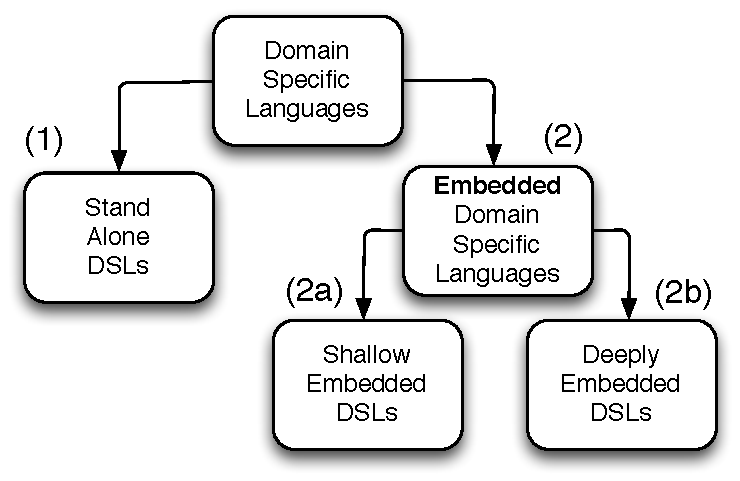
\includegraphics[width=0.4\textwidth]{images/TypesOfDSLs.pdf}
  \caption{Types of Domain Specific Languages}
  \label{fig:types-of-dsls}
\end{figure}
        
\section{Haskell Primer}

An Embedded DSL (EDSL) is a language inside a language.
Haskell~\cite{Haskell98Book}, the premier pure functional programming language, is a great host for EDSLs
because of flexible overloading, a powerful type system, and lazy semantics facilitating this.
In this section, we give a terse
introduction to Haskell, 
sufficient to make this article self-contained. This section was
adapted from the Haskell primer given in~\cite{?}.

Haskell is all about {\em types\/}. Types in Haskell, like
types in other languages, are constraining summaries of structural values.
For example, in Haskell \verb|Bool| is the type of the values
\verb|True| and \verb|False|, \verb|Int| is the type of machine-sized
words, \verb|Double| is the type of double precision floating
point values; and this list goes on in the same manner as
\verb|C|, \verb|C++|, \verb|Java| and other traditional languages.
All these type names in Haskell start with an upper-case letter.

On top of these basic types, Haskell has two syntactical forms for expressing
compound types.
First, pairs, triples and larger structures can be written using tuple syntax,
comma separated types inside parenthesis.
So \verb|(Int,Bool)| is structure with both an \verb|Int| and a \verb|Bool| component.
Second, lists have a syntactical shortcut, using square brackets.
So \verb|[Int]| is a list of \verb|Int|.

Haskell also has other container types. A container
that {\em may\/} contain one \verb|Int| has the type
\verb|Maybe Int|
which is read \verb|Maybe| of \verb|Int|.
These container names also start with upper-case letters.
Types can be nested to any depth. For example, we can have a \verb|[(Maybe (Int,Bool))]|,
read as list of \verb|Maybe| of (\verb|Int| and \verb|Bool|).

Polymorphic values, which are analogous to the type \verb|Object| in Java,
or \verb|void*| pointers in C, are expressed using lower-case letters.
These polymorphic values can have constraints expressed over them,
using the Haskell equivalent of an object hierarchy.
Finally, a Haskell function that takes a list, and returns a list
is written as using an arrow: \verb|[a] -> [a]|.

We can now give an example of a Haskell function.%, the function \verb|sort|.
\begin{Code}

sort :: (Ord a) => [a] -> [a]
sort []     = []
sort (x:xs) = sort before ++ [x] ++ sort after
  where
        before = filter (<= x) xs
        after  = filter (> x) xs

\end{Code}
This function sorted a list, using a variant of quicksort in which the pivot is
the first element of the list.
\begin{itemize}
\item The first line is the type for \verb|sort|. This is $\forall$\verb|a|, such that
\verb|a| can be \verb|Ord|ered (admits comparisons like \verb|<=|), the function
takes and return a list of such \verb|a|'s.
\item The second line says that an empty list is already sorted.
\item The remaining lines state that a (non-empty) list can be
sorted by taking the first and rest of the list (called \verb|x| and \verb|xs|, respectively),
and sorting the values before this pivot and after this pivot,
and concatenating theses intermediate values together.
\item Finally, intermediate values can be named using the \verb|where| syntax;
in this case the values of \verb|before| and \verb|after|.
\end{itemize}

Haskell is a concise and direct language.
Structures in Haskell are denoted using types, constructed
and deconstructed, but never updated. For example, the \verb|Maybe| type
can been defined using two constructors, \verb|Nothing|, and \verb|Just|.
\begin{Code}
        
data Maybe where
  Nothing ::      Maybe a
  Just    :: a -> Maybe a

\end{Code}
\verb|Nothing| is a verb|Maybe| of anything, \verb|Just|, with an argument,
is a \verb|Maybe| with the type of the argument. These constructors can be
used to construct and deconstruct structures, but there is never any updating;
all structures as immutable.

It is possible to give specific types extra powers, like equality and comparison,
using the class based overloading system. In the case of \verb|Maybe|, we
can give the \verb|Maybe| type the ability to test for equality, using an
instance.
\begin{Code}
instance Eq a => Eq (Maybe a) where        
   Just a  == Just b  = a == b
   Nothing == Nothing = True
   \_       == \_       = False
\end{Code}

This states that for any type that can be testing for equality,
we can also check \verb|Maybe| at the same type. We take the \verb|Maybe|
apart, using pattern matching on \verb|Just|, to check the internal value.a

In Haskell, Side-effects such as writing to the screen
or reading the keyboard are described using a \verb|do|-notation, for example:

\begin{Code}

main :: IO ()
main = do
  putStrLn "Hello"
  xs <- getLine
  print xs

\end{Code}

In this example a {\em value\/} called \verb|main| uses the \verb|do|-notation to describe
an interaction with a user. Actually, the \verb|do|-notation captures
this as a structure called a Monad; purity is not compromised. For more details
about how \verb|do|-notation and Monads can provide an effectful interface
inside a pure language like Haskell, see~\cite{SPJ:93:IFP}. For the
purposes of this article, \verb|do|-notation is a way of providing syntax
and structure that looks like interaction. There are many tutorials
on Haskell, but the Haskell website, \verb|haskell.org| is a good starting point
for further reading.

\section{Embedded DSLs}

An EDSL is a library in a host language which has the look, feel and semantics of its own language,
customized to a specific problem domain.
Using Haskell's concise syntax, Haskell specifically and the functional programming
community in general have taken the ideas
of EDSLs, which considerably lowered the costs of developing
and maintaining a DSL, and developed many, many of DSL 
which provide higher-level interfaces and abstractions for well-understood systems.

We look at two examples of DSLs, one for automatically generating test cases for software testing,
and a second for specifying hardware circuit behaviors.

\subsection{Example EDSL: QuickCheck Properties}

As a first example of a EDSL, consider the challenge of writing test cases.
Or more specifically, writing the {\em properties\/} that test cases need to satisfy.

\begin{Code}
-- The reverse of a reverse'd list is itself
prop_reverse_twice (xs :: [Int]) = reverse (reverse xs) == xs
\end{Code}

\verb|prop_reverse_twice| is a regular Haskell function,
that takes a list of Int, and returns a boolean, based
on the validity of what is being proposed, specifically
that is a two reverses cancel each other out. 
Here is the neat part -- \verb|prop_reverse_twice| is {\bf also\/} a
domain specific statement, and as such can also be considered
a sub-language inside of Haskell itself.  This style
of using functions, in this case function with names
prefixed with \verb|prop_|, taking a number of typed
arguments, and returning a conditional is a small language.
The property written in Haskell is also an Embedded Domain Specific
Language for properties.

We can run our EDSL, using a function called \verb|quickCheck|:
\begin{Code}
Prelude Test.QuickCheck> quickCheck prop_reverse_twice
+++ OK, passed 100 tests.
\end{Code}
By running \verb|quickCheck| with our explicit and specific property,
we execute our ESDL inside Haskell. The quickCheck function
generates 100 test cases for our property, and executes
them on the fly. If they all hold, then the system prints
a message reflecting this. The test cases are generated using
the type class system -- QuickCheck gives specific types the
power of test-case generation -- and the \verb|quickCheck| function
uses this to generate random tests.

Properties are useless unless they are falsify-able. As an examples
of an incorrect property, consider this property for reverse.
\begin{Code}
prop_reverse xs ys = reverse xs ++ reverse ys == reverse (xs ++ ys)
\end{Code}
This is stating that the reverse of two distinct lists
is the same as the reverse of both lists appended together.
But this property is false.
\begin{Code}
Prelude Test.QuickCheck> quickCheck prop_reverse 
FALSE!!!
\end{Code}

In turns out that this sort of mini-language is really useful in practice.
Despite the simplicity of how Haskell is being used, the QuickCheck EDSL
provided a way of thinking about and directly expressing properties.
In the full QuickCheck EDSL has additional functionality, including
the ability to generate random function arguments, the ability to control
the distribution of the random test cases, and the ability to state pre-conditions
to a property. From this language, several other implementations of
these idea have been constructed. There is even a swedish company, ???,
which sells a QuickCheck for Erlang, a language for large scale concurrency
as found in telephone switches, and the language used by snapchat, the recent
Facebook \$19 billion dollar purchase.

\section{Example EDSL: Kansas Lava}\label{sec:KansasLava}

To take another example, consider describing hardware.
Hardware description languages and functional languages have
long enjoyed a fruitful partnership.
{\bf Lava} is the name given to a class of Haskell DSLs
that implement a function-based version of the hardware description
language Ruby~\cite{Jones:90:Ruby,Hutton:93:RubyInterp}. Ruby, not to be confused with the
modern programming language with the same name, was based
on relations, not functions, and was inspired by
the seminal work in $\mu$FP~\cite{Sheeran:84:muFP}.

Kansas Lava~\cite{Gill:13:TypesKansasLava} is a Haskell-hosted DSL
that follows the Lava line of research.
Kansas Lava is a language for expressing gate-level circuits.
Haskell abstractions allow the programmer to work at
a slightly higher level of abstraction, where the model
is one of recursive components communicating via synchronized streams.
Kansas Lava has been deployed for the generation of high-performance circuits for telemetry decoders,
though the model used is general.

As an example of Kansas Lava, consider:

\begin{Code}

counter :: (Rep a, Num a, Clock clk, sig ~ Signal clk) => sig Bool -> sig Bool -> sig a
counter restart inc = loop
   where reg = register 0 loop
	 reg' = mux2 restart (0,reg)
	 loop = mux2 inc (reg' + 1, reg')
\end{Code}

This circuit connects two multiplexers (\verb|mux2|),
an adder,
and a \verb|register|
to give a circuit that counts the number of
clocked pulses on a signal \verb|inc|.
The circuit takes two clocked signals,
and returns a clocked signal that explicitly
operates using the same clock, because they
share the same type.
The use of arithmetic is understated,
but simply uses (via overloading) the
standard syntax for addition; the {\tt Num}
constraint allows this.
Figure~\ref{fig:counter-picture} gives the
circuit intended for this description.

\begin{figure}[!t]
    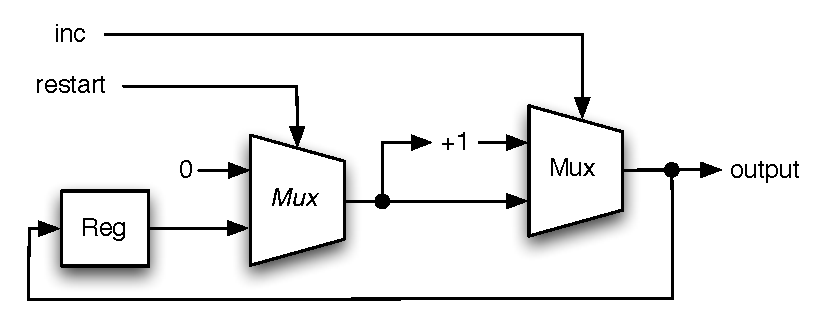
\includegraphics[width=0.4\textwidth]{images/Counter.pdf}
  \caption{{\tt counter} Schematic Kansas Lava parity counter}
  \label{fig:counter-picture}
\end{figure}


We can simulate sequential circuits with the
same directness as the combinational functions we invoked.
\begin{Code}
GHCi> toSeq (cycle [True,False,False])
T : F : F : T : F : F : T : F : F : ...
GHCi> counter low (toSeq (cycle [True,False,False]))
1 : 1 : 1 : 2 : 2 : 2 : 3 : 3 : 3 : ...
\end{Code}

As well as basic signal types,
we can build circuits that operate on Haskell
functions directly, provided the domain of the
function is finite. We use the \verb|Rep|
capability to signify that we can enumerate
all possible representable values in a type,
giving the \verb|funMap| function.
\begin{Code}
funMap :: (Rep a, Rep b, Clock c, sig ~ Signal c) => (a -> Maybe b) -> sig a -> sig b
\end{Code}
The generated circuit is implemented using a ROM,
and we can generate control logic
directly in terms of Haskell functions
and data-structures. As a example, consider
a small ROM that stores the square of a
value.
\begin{Code}
squareROM :: (Num a, Rep a, Clock c, sig ~ Signal c) => sig a -> sig a
squareROM = funMap (\ x -> return (x * x))
\end{Code}
In this way, direct Haskell functions
can be lifted into the \verb|Signal| world.
Notice how the \verb|squareROM| function is
not specific about size but is
completely generic, only requiring the
type of the argument stream
to be representable as a number.

We can now use our clock squaring ROM at specific types,
for example at 8-bit we can generate the follows.
\begin{Code}
GHCi> squareROM (toSeq [0,1..])        
0 : 1 : 4 : 9 : 16 : 25 : 36 : 49 : 64 : 81 : 100 : 121 : 144 : 169 : 196 : 225 : 0 : ...
\end{Code}

This level of circuit specification has been used to great
effect in many Lava and Lava-like languages. One notable
instance is Hawk, a Lava-like EDSL which was used to specify
the entire micro-architecture of the Pentium-Pro, including the
super-scaler design, and register bypass capabilities.

If DSLs are so powerful as an idiom for library design, then why have the taken over?
As a means for expressing things that can be {\em simulated\/}, EDSLs are an invaluable
design pattern. There are many, many examples, including ....

Not everything is a simulation. What if we wanted to use an EDSL to express
something that we want to run somewhere else, not inside the Haskell system?
Can we use Lava to generate circuits, and run them on FPGAs? Can we use EDSL
to generate code for embedded processors, or GPUs? Such an ability, to 
synthesis external solutions, would be extremely useful. We can extend
the EDSL idiom to do so, with significant caveats. The remainder of this
paper is about how we capture and offshore work from inside a EDSL, what
this capability can be used for, and what the limitations are.

\subsection{Deeply Embedded Domain Specific Language}

EDSLs are simply a way of thinking about a library
of provided functions, often called combinators, because they combine
their arguments into terms inside the DSL language and types. In our
Lava example above, the \verb|register| combinator takes an initial
value, and a incoming stream of values, and gives the new stream,
delayed by a single cycle, with the initial value occupying the initial
cycle. Critically, \verb|register| is compositional; it combines
smaller parts of the DSL to make larger solutions. If a DSL
follows this composability carefully by design, an alternative implementation
is possible.

The most common flavor of DSL is one  that uses a so-called shallow embedding, where values are computed with directly.
The result of a computation in a shallow DSL is a value. All the examples so far are shallow.
But there is another class of DSLs, 
specifically {\em DSLs that use a deep embedding\/} build an abstract syntax tree~\cite{Elliott:03:CompileDSEL-JFP}.
The result of a computation inside a Deeply Embedded DSL (Deep EDSL)
is a structure, not a value, and this structure can be used to compute a value,
or be cross-compiled before being evaluated. Such ``Deep'' EDSLs
follow the composability mantra pedantically, by design and mandate.

Historically, EDSLs have been shallow; simply a way of structuring an API to a library. 
However, Deep EDSLs have the ability to {\em stage\/} code, that is executing a program
can generate another program, much like the well-known YACC DSL,
but at the cost of significantly restricting what forms of the DSL can
generate valid output from.
There is a growing number of Deep EDSLs, and a body of research around their
form and limitations.
The unifying theme is that Deep EDSLs can be pragmatic, productive and useful.

In this section, we will investigate the basic structure of Deep EDSL compared to Shallow EDSLs,
and look at three pragmatic tricks for improving the usefulness of Deep EDSLs.

\subsection{Building a Deep EDSL}

A deeply embedded DSL is a DSL that exposes its own structure.
Rather than functions operating on a datastructure (a shallow DSL),
a deep DSL build a structure, and allows some secondary agent to
provide interpretation of this structures.
To make this idea concrete, consider a DSL for arithmetic,
with addition, subtraction, multiplication, and constants.
We want to be able to {\bf run\/} this DSL. For a shallow
embedding this is trivial - we just use the built in 
arithmetic. A deep embedding is where things get
interesting. Consider a data-type for our arithmetic.

\begin{Code}
data E where
 Lit :: Integer -> E
 Add :: E -> E -> E
 Sub :: E -> E -> E
 Mul :: E -> E -> E
 deriving Eq
\end{Code}

Now we overload the arithmetic to use this E datatype;
in Haskell Num is our overloading for integral arithmetic.

\begin{Code}
instance Num E where
  fromInteger n = Lit n
  e1 + e2 = Add e1 e2
  e1 - e2 = Sub e1 e2
  e1 * e2 = Mul e1 e2
\end{Code}

Now, if we build expressions of type E, we can
observe the structure of the computation.
\begin{SemiCode}
GHCi> 1 + 2 * 3
Mul (Add (Lit 1) (Lit 2)) (Lit 3)
\end{SemiCode}

This profound, and the key idea that makes deep embeddings work. We can written
an expression, and extracted a tree of {\em what\/} to do, not a direct result.
With deep embeddings, it is common to also
write a run function, that computes the structure
of a captured computation, given a simple value.
\begin{Code}
run :: E -> Int
run (Lit n) = n
run (Add a b) = run a + run b
run (Sub a b) = run a - run b
run (Mul a b) = run a * run b
\end{Code}

\begin{figure}[!t]
  \centering        
  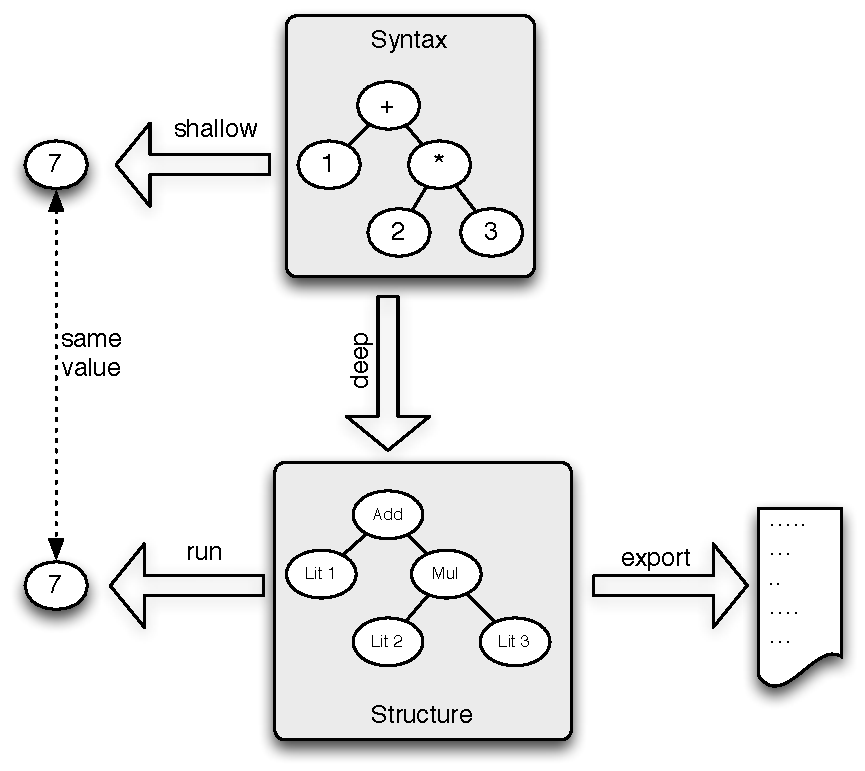
\includegraphics[width=0.6\textwidth]{images/DeepEmbedding.pdf}
  \caption{Shallow and Deep Embedding of Arithmetic}
  \label{fig:deep-dsls}
\end{figure}

Figure~\ref{fig:deep-dsls} illustrates the differences between shallow and deep DSLs,
and how a deep embedding combined with a specific run function gives the same result.
For a deep embedded DSL, the run function restores the capability of the shallow
embedding, but another function takes the embedded structure, and uses in in some creative way. 

In order to make deep DSLs practical, there are two folklore tricks that are used almost
always used.
First, we can capture functions, by using dummy arguments. Second, we can observe loops,
buy using some form of observable sharing. 
%And finally, we call observe imperative statements, by using normalization. 
%We will overview both these tricks, before concluding with shortcomings, extensions, and remaining challenges.

\subsection{How to extract a deep embedding from a function}

Expressing function calls in terms of constructors,  and
building expression trees is a useful, but by itself is a gimmick. 
However, with careful construction, we can also capture function definitions,
and other synaxtically structures,
directly from a deep embedding. It is at this
point, the idea of capturing code,
the using the captured code to execute code
on a different target becomes possible.
Consider a simple function to add one to its argument.

\begin{Code}

f :: E -> E
f x = x + 1
        
\end{Code}

Here we have a function that acts over our new type
\verb|E|, and returns a new \verb|E|. How can we capture
this function?
The trick is to invent a unique E, and pass it as a (dummy) argument
to \verb|f|.

\begin{Code}
data E where
  Lit :: Integer -> E
  ...
  Var :: String -> E    -- new constructor
\end{Code}        

\begin{Code}
-- Just running the function
> f 4
Add (Lit 4) (Lit 1)
-- reifing the function, using our unique E ``Var''.
> f (Var "x")
Add (Var "x") (Lit 1)   -- reified version of the function
\end{Code}

This is remarkable! We're run a function with 
a dummy argument (called the prototypical argument)
and extracted the body of the function.

There are many places this design pattern can be used. One example is the specification
of surface textures as functions; it is possible to export these into code executable
on GPUs, simultaneously lifting the abstractions used to write textures, and speeding
up how fast a shallow embedding of the same operations would run.  There is nothing
that is specific about Haskell, or even functional languages here. Indeed, the same
ideas have been used in Java, for a VHDL generator. Haskell, with its powerful abstractions,
allows deep DSLs to almost feel like a straightforward shallow embedding.

\subsection{How to spot a loop}

Lava programs are written as equations of recursive bindings.
If we attempt to build a deep embedding of Lava directly,
we will get into a infinite cycle of structures. In order to illustrate
the challenge, we will build a deep embedding of Lava,
see where it goes wrong, and fix it using a technique called
observable sharing.

First we need a structure for our Lava Language. We define the
functions use above, but give then a deep embedding, called \verb|Signal|.
\begin{Code}
        
data Signal where
  Register :: a -> Signal clk a                  -> Signal clk a
  Mux2     :: Signal Bool -> (Signal a,Signal a) -> Signal clk a
  Var      :: String                             -> Signal clk a -- the Var trick

mux2 :: Signal clk Bool -> (Signal a,Signal a) -> Signal a
mux2 c (a,b) = Mux2 c (a,b)

toSeq :: a -> Signal a
toSeq = ...

\end{Code}
Now, if we attempt to extract \verb|counter|, things go horribly wrong.
\begin{Code}
GHCi> counter (Var "restart") (Var "inc")
((( LOOPING CODE ))))
\end{Code}        
What has happened is the recursive definitions are unrolling when we try reify the function,
or more specifically, the body of counter is looping. At this point, the EDSL community was
stymied. There was efforts to use monadic structure, where the loop was expressing using
\verb|do|-notation~\cite{...}, making the loop an observable effect. There was an unsafe
extension to observe a limited form of sharing, by circumventing part of the purity of Haskell,
called observable sharing.
There was also an extension of Haskell input/output mechanism that allowed loops to
be observed indirect, called IO-based observable sharing. The net effect of all three
mechanisms is that the observed tree is rendered as a graph with named edges.

\begin{figure}[!t]
  \centering
   \begin{minipage}{0.5\textwidth}
     \centering
\footnotesize\begin{Code}[fontsize=\tiny]
entity counter is
  port(rst : in std_logic;
       clk : in std_logic;
       clk_en : in std_logic;
       restart : in std_logic;
       inc : in std_logic;
       output : out std_logic_vector(3 downto 0));
end entity counter;
architecture str of counter is
  signal sig_2_o0 : std_logic_vector(3 downto 0);
  ...
begin
  sig_2_o0 <= sig_5_o0 when (inc = '1')  else sig_6_o0;
  sig_5_o0 <= std_logic_vector(...);
  sig_6_o0 <= "0000" when (restart = '1') else sig_10_o0;
  sig_10_o0_next <= sig_2_o0;
  proc14 : process(rst,clk) is
  begin
    if rst = '1' then
      sig_10_o0 <= "0000";
    elsif rising_edge(clk) then
      if (clk_en = '1') then
        sig_10_o0 <= sig_10_o0_next;
  ....
end architecture;
\end{Code}
  \end{minipage}
  \caption{{\tt counter} Schematic and VHDL Generated by Kansas Lava}
  \label{fig:counter-pictureX}
%  \vspace{-0.1in}
\end{figure}

Haskell at this point rescues complexity. Advanced type-system mechanisms, such has higher-kind type
arguments, allow a structure to be either a tree or graph, depending on type-level instantiation. 
Omitting here the details, the reified function is a tree with sharing,
then translated into a graph with explicit sharing. The final result for our example is
\begin{Code}
GHCi> reify (counter (Var "restart") (Var "inc"))
[(0,REGISTER False 1),
 (...)
]
\end{Code}
In this output, each upper-case constructors correspond to its deep-embedding constructor.
A quick inspection shows that we have captured the circuit as given in Figure~\ref{counter-picture}.
From this netlist-style structure, it is straightforward to generate VHDL. For the example
of 4-bit number, the VHDL is given in Figure~\cite{counter-picutureX}.

These two tricks (prototypical argument, IO-based observable sharing) are the technical fundamentals
of Kansas Lava. On top of this base, and with help from Haskell type system, an entire ecosystem
for circuit generation has been developed. The DSL idiom allows programmers to use high-level 
abstraction, in Haskell, and generate efficient circuits. But not all is rosy; writing a Lava
program is not the same as writing a Haskell program because of the limitations of Deep
embeddings.

\subsection{A deep embedding is only half a program}

The basis of a Deep EDSL is one of constructiveness.
Functional programming is about constructing {\em and destructing\/} values.
Because of this, a deep embedding can not reify any pattern matching, 
or even direct usage of if-then-else, and other control flow. We side-stepped this
in Kansas Lava, for example by using a \verb|mux2| constructor, 
which encodes choice.

How much further can the idiom be pushed, if we need to be constructive?
The result is surprising. We start with our three capabilities:
\begin{itemize}
\item Basic expressions can be captured, by constructing a tree that is an analog to our syntax.
\item Functions can be captured, using the a fake unique argument.
\item Local bindings can be observed using some form of observable sharing.
\end{itemize}
With these three comes and automatic forth capability.
\begin{itemize}
\item MACRO EXPAND
\end{itemize}

There are also extensions to the basic techniques. The principle once are:
\begin{itemize}
\item Internal function calls can captured as notes on a graph, 
rather than directly inlined~\cite{...}. 
This helps compilation of large programs, giving a basic separate compilation capability.
\item \verb|do|-statement can be reified, by normalization~\cite{...}. This result, called monadic
reification, is surprising. There are strong technical reasons to be believe monadic reification
should be impossible. However the normalization refactors the constraining that, by themselves would
be impossible to solve, and matches them up, 1-on-1, with a matching solution, allowing the whole
\verb|do|-notation to be solved and reified.
Monadic reification is a recent discovery, but has already been used in several Deep DSLs,
including feldspar, and Sunroof.
\item Control flow is problematic, and can not be used directly. However,
there is a generalization of Haskell boolean that do allow deep embedding capture~\cite{boolean}.
Using this library, a DSL with control flow can be constructed, but it needs to be explicit
code, at the DSL level, using constructors.
\end{itemize}

So where does this leave Deep DSLs? They are clearly a useful tool for the
language implementor, but come with costs and limitations. How can we therefore
push the state of the art, and allow more of the Haskell language to reified?
There are two primary shortcoming.
One we have discussed already: control flow and pattern matching remain a thorn in Deep DSLs. 

Parametric polymorphism, one of the strengths of functional program, is the other
issue for deep DSLs. We need a specific structure to represent what we have captured,
and arbitrary polymorphism interferes with this. Current system sidestep this
by always instantiate at a specific type, but this expensive because size of
the captured program can expand exponentially.
Polymorphism was the technical reason that it was thought that monadic reification
would not work, but in that case it was side-stepped by normalization; this technique
does not generalize to all polymorphism.

Deep DSLs is the value-level way of extracting an expression, but there are others.
Quaziquoting is another, at the syntactically level. Haskell comes with an extensive
template system, called Template Haskell, that can and is used for DSLs.
(....)
Perhaps the future of Deep DSLs is some hybrid between expression generation
and quazi-quoting, combining the best of both systems.


\end{document}

% TODO: Something about code to generate DSL; automatic macros